\section{RQ1: Accuracy as the Catalog Grows}
\label{sec:rq1}

\begin{figure}[t]
  \centering
  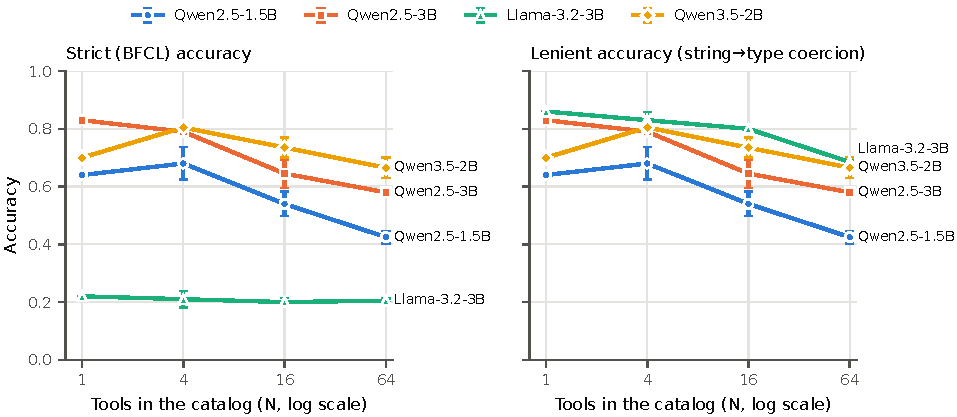
\includegraphics[width=\linewidth]{figures/fig_scaling.pdf}
  \caption{Accuracy against catalog size $N$ on 100 BFCL \texttt{simple\_python} queries (mean over two catalog seeds; error bars are standard deviations). Left: strict BFCL scoring. Right: lenient scoring, which converts string-encoded numbers and booleans to the schema type before checking. Llama-3.2-3B writes nearly every number as a string; its strict curve stays flat near 20\% and hides a clear decline.}
  \label{fig:scaling}
\end{figure}

\begin{table}[t]
  \centering
  \caption{Accuracy (\%) by catalog size (mean $\pm$ std over two catalog seeds, 100 queries each). $\Delta$ is the change from $N{=}1$ to $N{=}64$.}
  \label{tab:accuracy}
  \small
  \begin{tabular}{lccccc}
\toprule
Model & $N{=}1$ & $N{=}4$ & $N{=}16$ & $N{=}64$ & $\Delta_{1\to64}$ \\
\midrule
\multicolumn{6}{l}{\textit{Strict (BFCL) accuracy, \% (mean $\pm$ std over 2 catalog seeds)}} \\
Qwen2.5-1.5B & 64.0 & 68.0\,$\pm$\,5.7 & 54.0\,$\pm$\,4.2 & 42.5\,$\pm$\,2.1 & -21.5 \\
Qwen2.5-3B & 83.0 & 79.0 & 64.5\,$\pm$\,4.9 & 58.0\,$\pm$\,1.4 & -25.0 \\
Llama-3.2-3B & 22.0 & 21.0\,$\pm$\,2.8 & 20.0\,$\pm$\,1.4 & 20.5\,$\pm$\,0.7 & -1.5 \\
Qwen3.5-2B & 70.0 & 80.5\,$\pm$\,0.7 & 73.5\,$\pm$\,3.5 & 66.5\,$\pm$\,3.5 & -3.5 \\
\midrule
\multicolumn{6}{l}{\textit{Lenient accuracy, \% (string-encoded scalars coerced to schema type)}} \\
Qwen2.5-1.5B & 64.0 & 68.0\,$\pm$\,5.7 & 54.0\,$\pm$\,4.2 & 42.5\,$\pm$\,2.1 & -21.5 \\
Qwen2.5-3B & 83.0 & 79.0 & 64.5\,$\pm$\,4.9 & 58.0\,$\pm$\,1.4 & -25.0 \\
Llama-3.2-3B & 86.0 & 83.0\,$\pm$\,2.8 & 80.0 & 68.5\,$\pm$\,0.7 & -17.5 \\
Qwen3.5-2B & 70.0 & 80.5\,$\pm$\,0.7 & 73.5\,$\pm$\,3.5 & 66.5\,$\pm$\,3.5 & -3.5 \\
\bottomrule
\end{tabular}
\end{table}

\Cref{fig:scaling} and \cref{tab:accuracy} show the main result.
\textbf{Every model loses accuracy as the catalog grows, and the loss is already large at 16 tools}, far below the hundreds of tools studied for larger models \citep{kate2025longfunceval}.
From $N{=}1$ to $N{=}64$, Qwen2.5-3B drops from \AccQwenThreeNOne\% to \AccQwenThreeNSixtyFour\% ($-$\DropQwenThree{} points) and Qwen2.5-1.5B from \AccQwenOneFiveNOne\% to \AccQwenOneFiveNSixtyFour\% ($-$\DropQwenOneFive{} points). Both drops are significant in paired McNemar tests ($p$\,\McNemarPQwenThree{} and \McNemarPQwenOneFive).
Up to four tools, accuracy is essentially flat: the differences between $N{=}1$ and $N{=}4$ are within the noise of 100 queries. The decline starts between 4 and 16 tools.

Two models need a closer reading.
\emph{Llama-3.2-3B} looks insensitive to $N$ under strict scoring (\AccLlamaNOne\% $\to$ \AccLlamaNSixtyFour\%; $p$\,=\,\McNemarPLlama). The reason is that it serialises numbers and booleans as strings (\texttt{"base": "10"}), which BFCL counts as type errors. Lenient scoring raises its accuracy by \LenGainLlama{} points on average and reveals the same decline as the Qwen models: \LenLlamaNOne\% $\to$ \LenLlamaNSixtyFour\% ($-$\LenDropLlama{} points).
\emph{Qwen3.5-2B} is \emph{better} with a few tools than with one (\AccQwenThreeFiveNOne\% at $N{=}1$, \AccQwenThreeFiveNFour\% at $N{=}4$). Given only one tool, it often answers arithmetic questions directly instead of calling the tool (\cref{sec:rq2}). From its best point at $N{=}4$ it then loses \DropFromBestQwenThreeFive{} points by $N{=}64$ ($p$\,\McNemarFourPQwenThreeFive).
Of the four models, Qwen3.5-2B degrades least at $N{=}64$, despite being the second-smallest. Its 8-bit weights, versus 4-bit for the others, are a possible confounder (\cref{sec:limitations}).

\paragraph{Position of the gold tool.}
At $N{=}64$, we see no consistent position effect (\cref{fig:position}, \cref{app:extra}). Accuracy varies non-monotonically across the four position quartiles. The two nominally significant tests (Llama, $p$\,=\,\PosPLlama; Qwen3.5, $p$\,=\,\PosPQwenThreeFive) do not survive a Bonferroni correction for four comparisons. With 64 tools, which is 8--10k tokens, these models do not show the lost-in-the-middle pattern reported for much longer contexts \citep{liu2024lost, kate2025longfunceval}. Our sample is small, so we only rule out large effects.

\paragraph{Cost.}
Prompt length grows linearly with $N$: about 250 tokens at $N{=}1$ and 8--10k tokens at $N{=}64$ (\cref{tab:cost}). Because queries that share a catalog reuse the key-value cache, the median latency per call stays low for the Qwen2.5 models (\LatQwenThreeNSixtyFour\,s for Qwen2.5-3B at $N{=}64$). For Llama-3.2-3B, whose cache does not fit in 4\,GB, it rises to \LatLlamaNSixtyFour\,s.
